\documentclass[11pt]{article}

\usepackage[final]{acl}

% Standard package includes
\usepackage{times}
\usepackage{latexsym}
\usepackage{booktabs}
\usepackage{graphicx}
\usepackage[T1]{fontenc}
\usepackage[utf8]{inputenc}
\usepackage{microtype}
\usepackage{inconsolata}
\usepackage{subcaption}
\usepackage{caption}

\title{From TF-IDF to Transformers: A Sentimental Journey through IMDb Reviews}

\author{Jiaxuan Guo \\
  Faculty of Engineering / The University of Tokyo \\
  Tokyo, Japan \\
  \texttt{jxguo@g.ecc.u-tokyo.ac.jp} }

\begin{document}
\maketitle
\begin{abstract}
This report presents a comparative study of three distinct paradigms for sentiment analysis on the IMDb movie review dataset. We implement and evaluate a classical machine learning model (TF-IDF with SVM), a recurrent neural network (Bidirectional LSTM), and a modern transformer-based model (fine-tuned DistilBERT). Our experiments quantify the trade-offs between these approaches in terms of performance, computational requirements, and implementation complexity. The results demonstrate that the fine-tuned DistilBERT model achieves a state-of-the-art accuracy of 89.20\%, while a simpler model like TF-IDF with SVM provides a strong and efficient baseline with 85.94\% accuracy. We also investigate the impact of model architecture and training duration for the LSTM model, identifying overfitting as a key challenge. This work concludes that the optimal choice of model is highly dependent on an application's specific constraints, including accuracy requirements, resource availability, and development time.
\end{abstract}

\section{Introduction}

Sentiment analysis, a key task in Natural Language Processing (NLP), involves determining the emotional tone or polarity of a piece of text. It has wide-ranging applications, from gauging customer feedback on products to monitoring public opinion on social media.

This project utilizes the well-known IMDb dataset \textit{(Introduced on Week 6's Lecture)}, which contains 50,000 movie reviews labeled as either positive or negative. Our primary objective is to provide a clear, hands-on comparison of three generations of NLP models for this binary classification task. By implementing each model, we aim to understand their theoretical underpinnings and practical trade-offs, offering insights into why and when to choose one approach over another.

\section{Models and Methodology}

We selected three different types of model, each representing a distinct era in NLP.

\subsection{Baseline: TF-IDF with SVM}
Our baseline model employs a classical machine learning pipeline. Text is first converted into numerical vectors using the Term Frequency-Inverse Document Frequency (TF-IDF) method. This approach represents each document as a vector of word importance scores, effectively a "bag-of-words" that captures word frequency but disregards word order. These vectors are then fed into a Linear Support Vector Machine (LinearSVC), a highly effective and efficient classifier for high-dimensional, sparse data.\textit{(Introduced on Week 3's Lecture)}

\subsection{Recurrent Neural Network: Bi-LSTM}
To capture the sequential nature of language, we implemented a Recurrent Neural Network (RNN) using a stacked Bidirectional Long Short-Term Memory (Bi-LSTM) architecture \textit{(Introduced on Week 9's Lecture)}. Our primary model begins with an Embedding layer that maps word indices to dense vectors. These are then processed by two sequential Bi-LSTM layers (e.g., 64-64 units) that read the text from both directions to capture rich contextual information. A Dropout layer is applied between the recurrent layers for regularization, and a final Dense layer with a sigmoid activation function produces the probability score for the positive sentiment class.

\subsection{Transformer-based Model: DistilBERT}
Representing the state-of-the-art, we utilized a transformer-based model, specifically DistilBERT, a smaller and faster version of BERT. This approach leverages the "pre-train and fine-tune" paradigm. The model is pre-trained on a massive corpus of text, endowing it with a deep, contextual understanding of language, which we then fine-tune on our specific IMDb dataset. The entire process was managed using the Hugging Face \texttt{transformers} library.

\section{Experiments and Results}

\subsection{Experimental Setup}
For all experiments, we used subsets of the IMDb dataset. For the SVM and LSTM models, we used 25000 training samples and 25000 test samples. For the DistilBERT model, we used 2,500 training samples and 500 test samples with 3 epochs to keep fine-tuning time manageable. We evaluated all models primarily on accuracy. All deep learning experiments were conducted on a Google Colab T4 GPU.

\subsection{Hyperparameter Tuning for LSTM}
To determine an optimal configuration for our Bi-LSTM model, we experimented with network depth and the number of training epochs. The results are summarized in Table~\ref{tab:lstm-tuning}.

\begin{table}[h!]
\centering
\resizebox{\columnwidth}{!}{%
\begin{tabular}{lcccc}
\toprule
\textbf{Architecture} & \textbf{Epochs} & \textbf{Best Val Acc.} & \textbf{Best at Epoch} & \textbf{Final Val Loss} \\
\midrule
LSTM (64-128-64) & 4 & 82.83\% & 4 & 40.43\% \\
LSTM (64-128-64) & 5 & 83.94\% & 5 & \textbf{36.96\%} \\
LSTM (64-128-64) & 10 & 85.05\% & 9 & 40.48\% \\
LSTM (64-128-64) & 20 & 82.92\% & 3 & 85.90\% \\
\midrule
LSTM (64-64) & 4 & \textbf{85.08\%} & 2 & 38.81\% \\
LSTM (64-64) & 10 & 83.43\% & 2 & 72.47\% \\
\bottomrule
\end{tabular}
}
\caption{Performance of LSTM models with different depths and epochs. Best validation accuracy shows the peak performance before significant overfitting.}
\label{tab:lstm-tuning}
\end{table}

The tuning process indicated that the shallower `64-64` architecture trained for 4 epochs yielded the highest validation accuracy of 85.08\%. We observed that longer training durations or deeper architectures did not necessarily lead to better generalization and often resulted in overfitting. Based on these findings, we selected this best-performing LSTM configuration for our final comparison.

\subsection{Overall Model Comparison}
We then compared the performance of our optimized Bi-LSTM against the TF-IDF+SVM baseline and the fine-tuned DistilBERT model. The final results are presented in Table~\ref{tab:final-comparison}.

\begin{table}[h!]
\centering
\begin{tabular}{lcc}
\toprule
\textbf{Model} & \textbf{Accuracy} & \textbf{Training Time} \\
\midrule
TF-IDF + SVM & 85.94\% & \textasciitilde5 sec \\
Bi-LSTM (Best) & 85.08\% & \textasciitilde2 min \\
DistilBERT & \textbf{89.20\%} & \textasciitilde7 min \\
\bottomrule
\end{tabular}
\caption{Final performance comparison of the three models, focusing on accuracy and training time (CoLab T4 GPU for each models).}
\label{tab:final-comparison}
\end{table}

The fine-tuned DistilBERT model significantly outperforms the other two approaches. The classical SVM approach provides a strong and fast baseline, slightly outperforming our best LSTM configuration in these experiments. This highlights the effectiveness of traditional methods and the challenges of training RNNs from scratch without extensive tuning.

\section{Discussion}
The experimental results highlight a clear trade-off between performance and resources. The TF-IDF + SVM model is incredibly efficient, requiring only a CPU and seconds to train, making it an excellent choice for baseline systems. The Bi-LSTM model introduces significant complexity and, while it understands word order, is prone to overfitting and requires a GPU for reasonable training times. The DistilBERT model demonstrates the immense power of transfer learning. By leveraging knowledge from its pre-training phase, it achieves a superior understanding of language, leading to the highest accuracy at the cost of greater computational requirements.

\section{Conclusion}
This study successfully compared three generations of NLP models for sentiment analysis. We confirmed that modern transformer-based models offer state-of-the-art performance, while classical methods remain highly relevant as efficient baselines. The choice of the "best" model is not absolute but is a function of a project's specific constraints. Future work could involve more extensive hyperparameter tuning and exploring larger transformer models.

\section*{Limitations}
This study was conducted on subsets of the full IMDb dataset to ensure rapid experimentation. The hyperparameter tuning was not exhaustive. The results, therefore, represent a practical comparison within a constrained environment rather than the maximum achievable performance of each model.

\appendix

\section{Bi-LSTM Training Visualizations}
\label{sec:appendix}

Figures~\ref{fig:lstm-64-64-curves} and~\ref{fig:lstm-64-128-64-curves} display the training and validation curves for the Bi-LSTM hyperparameter experiments, illustrating the onset of overfitting.

\begin{figure}[htbp]
  \centering
  \begin{subfigure}{0.3\textwidth}
    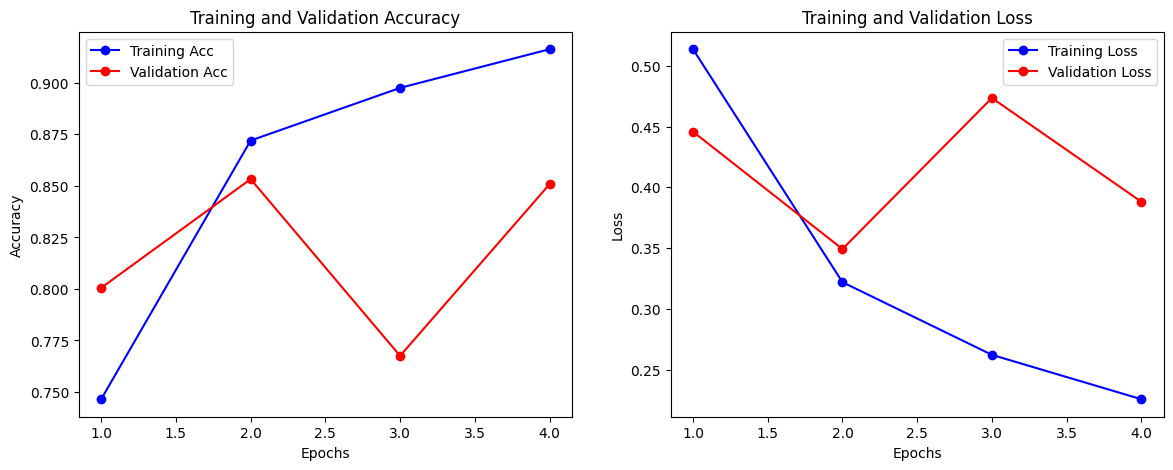
\includegraphics[width=\linewidth]{figs/4_2.png}
    \caption{64-64 Arch, 4 Epochs}
    \label{fig:lstm-64-64-4e}
  \end{subfigure}
  \hfill
  \begin{subfigure}{0.3\textwidth}
    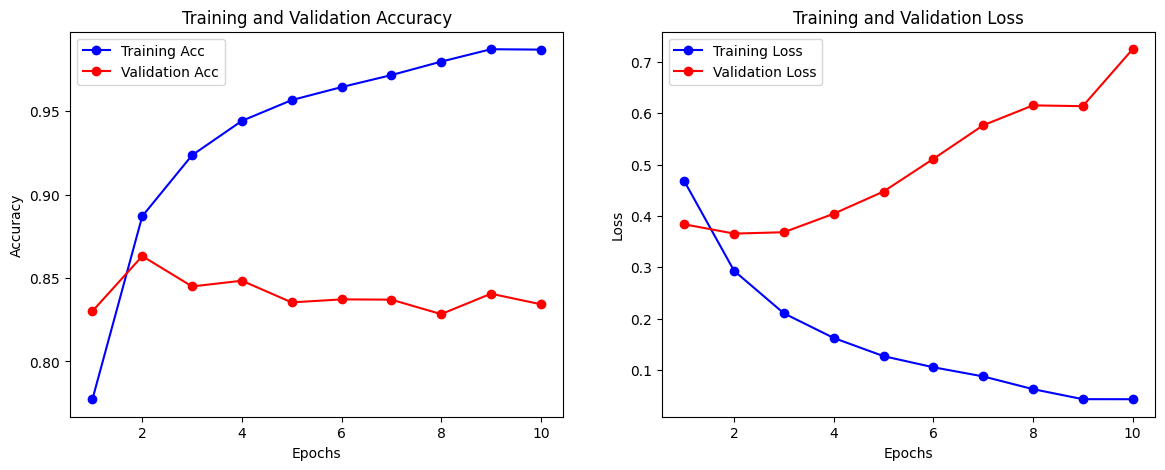
\includegraphics[width=\linewidth]{figs/10_2.png}
    \caption{64-64 Arch, 10 Epochs}
    \label{fig:lstm-64-64-10e}
  \end{subfigure}
  \caption{Learning curves for the shallower Bi-LSTM (64-64) architecture.}
  \label{fig:lstm-64-64-curves}
\end{figure}

\begin{figure}[htbp]
  \centering
  \begin{subfigure}{0.3\textwidth}
    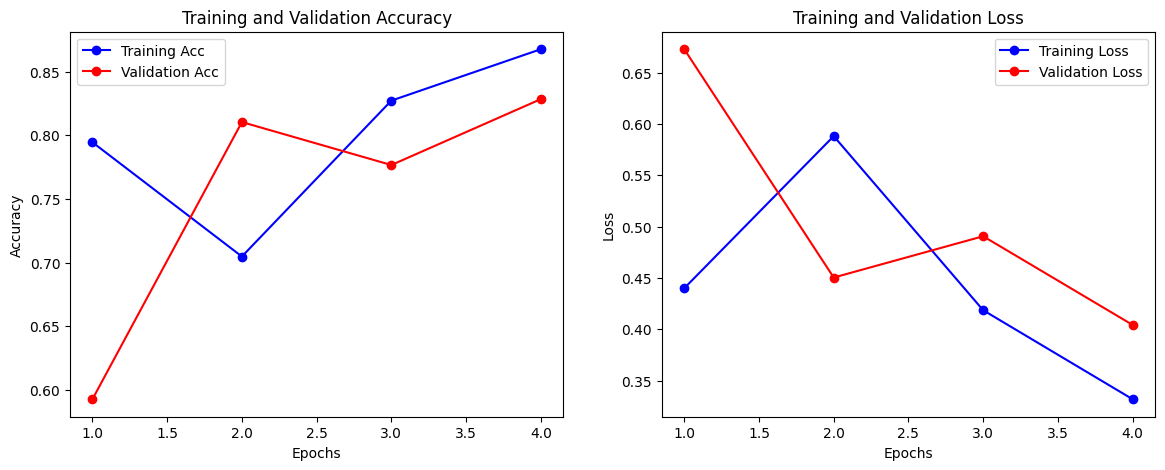
\includegraphics[width=\linewidth]{figs/4_3.png}
    \caption{64-128-64 Arch, 4 Epochs}
    \label{fig:lstm-64-128-64-4e}
  \end{subfigure}
  \hfill
  \begin{subfigure}{0.3\textwidth}
    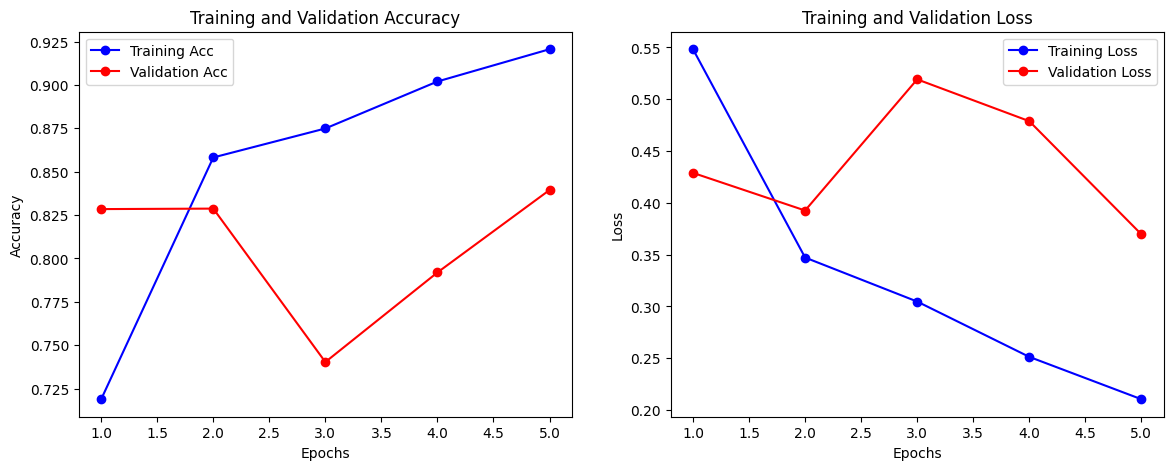
\includegraphics[width=\linewidth]{figs/5_3.png}
    \caption{64-128-64 Arch, 5 Epochs}
    \label{fig:lstm-64-128-64-5e}
  \end{subfigure}
  \hfill
  \begin{subfigure}{0.3\textwidth}
    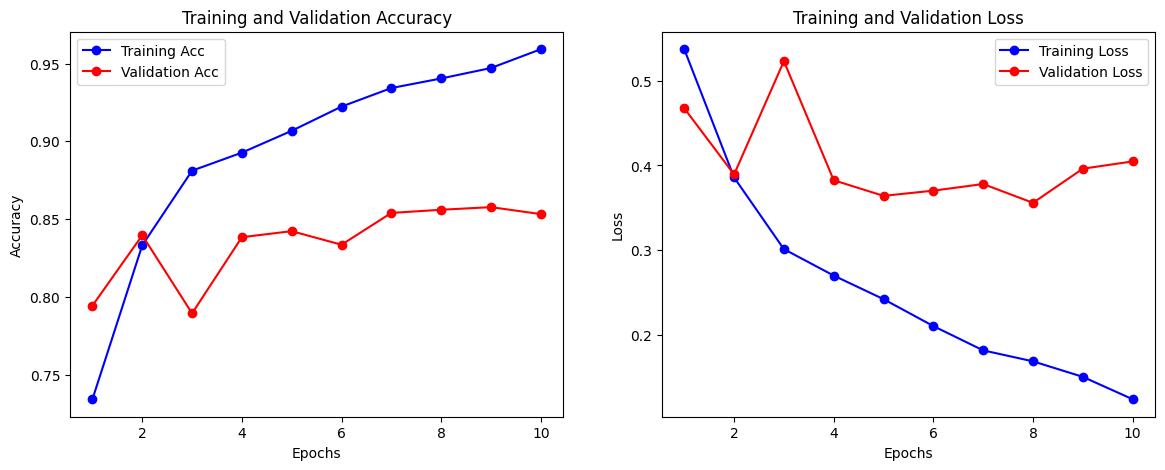
\includegraphics[width=\linewidth]{figs/10_3.png}
    \caption{64-128-64 Arch, 10 Epochs}
    \label{fig:lstm-64-128-64-10e}
  \end{subfigure}
 
  \caption{Learning curves for the deeper Bi-LSTM (64-128-64) architecture.}
  \label{fig:lstm-64-128-64-curves}
\end{figure}


\section{Fine-tuning Progress of DistilBERT}
\label{sec:appendix}

Table~\ref{tab:training-progress} shows the training progress of the DistilBERT model at various steps during the fine-tuning process.

\begin{table}[htbp]
  \centering
  \begin{tabular}{cccc}
  \toprule
  \textbf{Step} & \textbf{Training Loss} & \textbf{Validation Loss} & \textbf{Accuracy} \\
  \midrule
  50 & 0.694300 & 0.682717 & 0.534000 \\
  100 & 0.622700 & 0.461688 & 0.848000 \\
  150 & 0.360300 & 0.315430 & 0.874000 \\
  200 & 0.309800 & 0.316661 & 0.874000 \\
  250 & 0.260700 & 0.299690 & 0.880000 \\
  300 & 0.352700 & 0.285557 & 0.888000 \\
  350 & 0.178400 & 0.371934 & 0.884000 \\
  400 & 0.209900 & 0.258960 & 0.892000 \\
  450 & 0.195400 & 0.478180 & 0.844000 \\
  \bottomrule
  \end{tabular}
  \caption{Training progress of the DistilBERT model, showing loss and validation accuracy at different steps.}
  \label{tab:training-progress}
  \end{table}

\end{document}